\documentclass{article}
\usepackage[utf8]{inputenc}
\usepackage[cyr]{aeguill}
\usepackage[francais]{babel}
\usepackage{graphicx}



\title{Reconnaissance des espèces de plantes grâce à la forme de leurs feuilles}

\author{Marie Lavigne, Thibaud Levasseur, Nicolas Monet}

\begin{document}
\maketitle
\newpage
\tableofcontents
\newpage
\section{Introduction}
Actuellement le nombre d'espèces de plantes sur Terre est estimé à 310 000 - 420 000, dont beaucoup encore inconnues. Leur reconnaissance a toujours été un enjeu primordial pour les populations, tant pour leur survie par la reconnaissance des plantes comestibles ou empoisonnées, que pour la protection de l'environnement. \\
Différentes méthodes furent utilisées pour les classifier, allant de la morphologie à l'étude cellulaire en passant par la phytochimie. Cependant, les avancées technologiques des dernières décennies en informatique et notamment dans le domaine de la vision nous permettent à présent d'utiliser les ordinateurs pour de telles classifications. \\
\\
Dans ce cas, quelle partie de la plante demander à l'algorithme de reconnaître ?
Les fleurs ? Disponibles uniquement lors des floraisons, elles forment pour un ordinateur un objet complexe puisqu'en 3D et dont une simple photo ne saurait capter l'intégralité des singularités qui les composent. Ainsi les fleurs seraient trop complexes à traiter pour un temps de présence trop court. 
Le même raisonnement peut être tenu pour les fruit et l'écorce quant à elle n'est disponible que sur trop peu de spécimens. \\
Reste alors les feuilles, présentes chez la majorité des plantes et durant une période plus longue que les fleurs puisqu'elles ne disparaissent habituellement qu'en hiver. Les feuilles ont la particularité d'être presque toujours en 2D permettant, à l'aide d'une simple photo du dessus, un traitement très simple de ses spécificités. \\
\\
Maintenant que le sujet d'étude est défini, nous devons penser aux critères de reconnaissance d'une espèce. En imagerie, deux critères principaux peuvent nous venir en tête pour différencier des feuilles : la couleur et la forme. \\
Cependant, la couleur d'une feuille peut énormément varier, que ce soit en fonction du changement de saison qu'à cause de l'ensoleillement ou de l'humidité. Ce critère n'est donc pas assez fiable pour être utilisé parallèlement à la forme. Ainsi, les images utilisées ne nécessiteront que des nuances de gris. \\
L'objet de notre étude portera en conclusion principalement sur les formes de feuilles variés que possèdent chaque plante.
\paragraph{}
Ce projet a été réalisé grâce au travail des chercheurs Ji-Xiang Du, Xiao-Feng Wang et Guo-Jun Zang et notamment à leur article publié sur science-direct.com ( 185 (2007) 883–93). Les données utilisées sont quant à elles issues du site internet http://archive.ics.uci.edu/ml/datasets.html.
\newpage

\section{Description des données}
Le jeu de donné utilisé comporte 360 feuilles en images couleur et noir et blanc réparties et triées en 36 espèces. Le nombres d'individu par groupe est assez réduit et ne dépasse pas le nombre de 16. Une imprécision peut donc apparaitre dû au nombre réduit d'individu dans chaque échantillon.
\paragraph{}
Les images ont une résolution de 960*720 pixel, ce qui offre précision suffisante, sans être excessive. Cependant le temps de calcul pour la sérialisation des données reste assez long : quelques secondes par image. Une sauvegarde de celle-ci est donc fortement conseillée.
\paragraph{}
La représentation des feuilles est homogène : l'image est centrée et pour chaque feuille le pétiole est placé vers le bas de l'image, ce qui permet de faciliter grandement le traitement de l'image dans la mesure ou aucune rotation n'est nécessaire en pré-traitement.

\begin{center}
	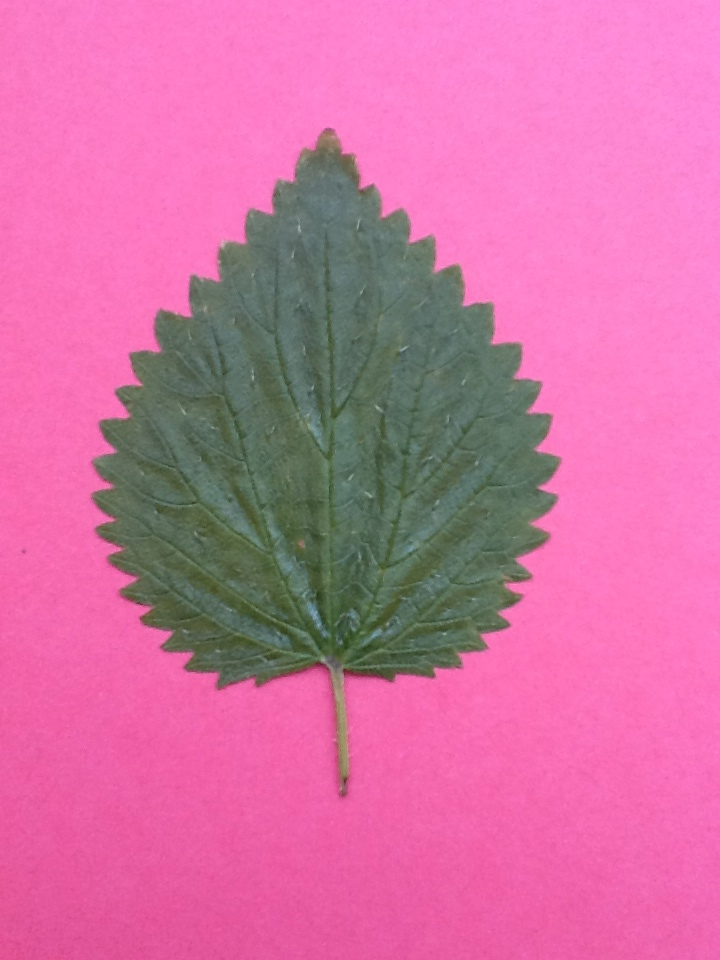
\includegraphics[scale=0.11]{image/urticaRGB.png}	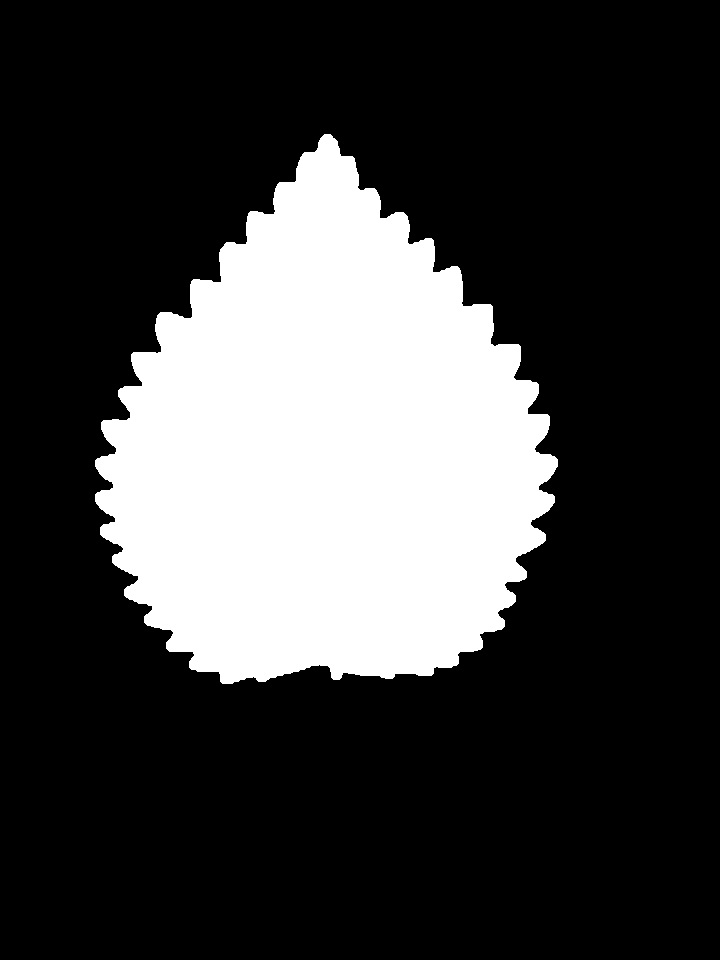
\includegraphics[scale=0.15]{image/urticaNB.png}
\end{center}
\section{Développement}
Le traitement de l'image est très basique: on charge une image en noir et blanc, on en trace le contour, et on calcule des paramètres propres à l'image (zones d'intéret, aire, périmètre...)
\smallbreak
Ce programme est basé sur l'apprentissage des formes, et sur du clustering. \\
On a une banque de données, des images de feuilles, qu'on traite pour calculer les paramètres décrits précédemment, et on labelle ces données: telle feuille a telles caractéristiques et c'est une feuille d'Erable, une autre a telles caractéristiques et c'est une feuille d'Ortie. \\
A partir de cet apprentissage on obtient des classes.
\smallbreak
Ensuite, on calcule les caractéristiques de la feuille à analyser. Par la méthode des KPPV (Plus Proches Voisins) on cherche la classe la plus proche de notre feuille, qui est la classe la plus ressemblante. \\
On détermine ainsi de quel type de feuille il s'agit.
\newpage
\section{Conclusion}
Avec nos données de test (16 et 12 feuilles de 2 types différents) on obtient 100 \% de réussite.\\
Le temps d'apprentissage est d'environ une seconde par image à traiter. \\
Le temps d'exécution est d'environ une seconde, qui est utilisé très majoritairement par la détermination des caractéristiques de la feuille. L'algorithme KPPV est relativement rapide et son temps d'exécution est négligeable en comparaison.
\newpage
\section{Annexes}
Concernant le code: le programme utilise une fonction TIMVecteur qui renvoie un vecteur avec les caractéristiques de l'image.

\end{document}
